\chapter{K"unstliche neuronale Netze (unfinished)}
{
- Ablauf: Training, Testing, Using?\\
- k"unstliche Intelligenz und Maschinen lernen\\
- Was k"onnen sie: label und prediction\\
http://deeplearning4j.org/neuralnet-overview\\
Neural networks are a set of algorithms, modeled loosely after the human brain, that are designed to recognize patterns. They interpret sensory data through a kind of machine perception, labeling or clustering raw input. The patterns they recognize are numerical, contained in vectors, into which all real-world data, be it images, sound, text or time series, must be translated.
They help group unlabeled data according by similarities among the example inputs, and they classify data when they have a labeled dataset to train on. To be more precise, neural networks extract features that are fed to other algorithms for clustering and classification.

\section{Feedforward Netzwerke (unfinished)}
Ein Feedforward Netzwerk besteht aus Layern und Neuronen. Die Neuronen sind f"ur die Berechnungen zust"andig w"ahrend die Layer den Aufbau des Netzes bestimmen. Abbildung 2.1 zeigt einen m"oglichen Aufbau eines k"unstliches Neurons.
\renewcommand{\figurename}{Abb.}
\begin{figure}[htp]
\centering
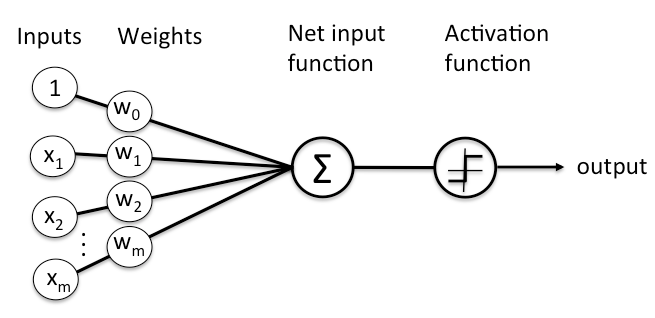
\includegraphics[width=0.60\textwidth]{pictures/perceptron_node.png}
\caption[Ein Neuron]{m"ogliches Aussehen eines Neurons\protect\footnotemark}
\end{figure}
\footnotetext{Quelle: DL4J \url{http://deeplearning4j.org/neuralnet-overview}}\\
Dieses Neuron besteht aus 1 bis x\textsubscript{m} Eing"angen (Inputs) mit Gewichten (Weights), einer Input Funktion (Net input function), einer Aktivierungsfunktion (Activation function) und einem Ausgang (Outputs). Die zu verarbeiteten Daten werden an die Eing"ange gelegt, durch die zugeh"origen Gewichte verst"arkt oder abgeschw"acht und anschlie{\ss}end aufsummiert. Die entstandene Summe wird dann an die Aktivierungsfunktion "ubergeben, welche das Ergebnis dieses Neurons festlegt.


Ein Layer besteht aus einer Reihe von Neuronen beliebiger Anzahl. Ein k"unstliches neuronales Netz setze sich aus einem Input Layer, einem Output Layer und beliebig vielen Hidden Layern zusammen. Hat ein Netz mehr als ein Hidden Layer so wird es auch als Deep Learning Netz bezeichnet.
\renewcommand{\figurename}{Abb.}
\begin{figure}[htp]
\centering
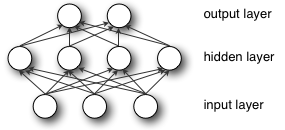
\includegraphics[width=0.50\textwidth]{pictures/mlp.png}
\caption[Aufbau eines Feedforward Netzes]{Aufbau eines Feedforward Netzes\protect\footnotemark} 
\end{figure}
\footnotetext{Quelle:  DL4J \url{http://deeplearning4j.org/neuralnet-overview}}\\
Abbilding 2.2 zeigt ein Feedforward Netzwerk. Bei diesem Netz besitzt das Input Layer drei Neuronen, das Hidden Layer hat vier und das Output Layer hat zwei Neuronen. Die Ergebnisse des Input und Hidden Layers dienen dem nachfolgenden Layer als Eingang.


Ein neuronales Netz kann anhand von Trainingsdaten eine Funktion erlernen, indem es die Gewichte ver"andert. Da bei Trainingsdaten das Ergebnis bekannt ist, muss das Netz die Gewichte so bestimmen, dass sie mit den Eingangsdaten den gew"unschten Ausgang mit m"oglichst kleinem Fehler abbilden. Das Ziel ist m"oglichst schnell den Punkt zu erreichen an dem der Fehler am kleinsten ist. Um dies zu erreichen wiederholt das Netz die folgenden Schritte: Ergebnis anhand der aktuellen Gewichte bestimmen, Fehler messen, Gewichte aktuallisieren.
Eine weitverbreitete Optimierungsfunktions zur Gewichtebestimmung hei{\ss}t Gradient Descent. Sie beschreibt das Verh"altnis des Fehlers zu einem einzelnen Gewicht und wie sich der Fehler ver"andert wenn das Gewicht angepasst wird.

Sources:\\
- http://deeplearning4j.org/neuralnet-overview\\


\section{Der Vorteil von Deep Learning (unfinished)}
- http://deeplearning4j.org/neuralnet-overview\\
In deep-learning networks, each layer of nodes trains on a distinct set of features based on the previous layer’s output. The further you advance into the neural net, the more complex the features your nodes can recognize, since they aggregate and recombine features from the previous layer.

This is known as feature hierarchy, and it is a hierarchy of increasing complexity and abstraction. It makes deep-learning networks capable of handling very large, high-dimensional data sets with billions of parameters that pass through nonlinear functions.

Above all, these nets are capable of discovering latent structures within unlabeled, unstructured data, which is the vast majority of data in the world. Another word for unstructured data is raw media; i.e. pictures, texts, video and audio recordings. Therefore, one of the problems deep learning solves best is in processing and clustering the world’s raw, unlabeled media, discerning similarities and anomalies in data that no human has organized in a relational database or ever put a name to.

For example, deep learning can take a million images, and cluster them according to their similarities: cats in one corner, ice breakers in another, and in a third all the photos of your grandmother. This is the basis of so-called smart photo albums.

Now apply that same idea to other data types: Deep learning might cluster raw text such as emails or news articles. Emails full of angry complaints might cluster in one corner of the vector space, while satisfied customers, or spambot messages, might cluster in others. This is the basis of various messaging filters, and can be used in customer-relationship management (CRM). The same applies to voice messages. With time series, data might cluster around normal/healthy behavior and anomalous/dangerous behavior. If the time series data is being generated by a smart phone, it will provide insight into users’ health and habits; if it is being generated by an autopart, it might be used to prevent catastrophic breakdowns.

Deep-learning networks perform automatic feature extraction without human intervention


\section{Recurrent Neuronal Networks (RNN) (unfinished)}
http://deeplearning4j.org/lstm.html
Recurrent networks, on the other hand, take as their input not just the current input example they see, but also what they perceived one step back in time.
The decision a recurrent net reached at time step t-1 affects the decision it will reach one moment later at time step t. So recurrent networks have two sources of input, the present and the recent past, which combine to determine how they respond to new data, much as we do in life.
Recurrent networks are distinguished from feedforward networks by that feedback loop, ingesting their own outputs moment after moment as input. It is often said that recurrent networks have memory.2 Adding memory to neural networks has a purpose: There is information in the sequence itself, and recurrent nets use it to perform tasks that feedforward networks can’t.
That sequential information is preserved in the recurrent network’s hidden state, which manages to span many time steps as it cascades forward to affect the processing of each new example.
Given a series of letters, a recurrent will use the first character to help determine its perception of the second character, such that an initial q might lead it to infer that the next letter will be u, while an initial t might lead it to infer that the next letter will be h.


https://colah.github.io/posts/2015-08-Understanding-LSTMs/
Humans don’t start their thinking from scratch every second. As you read this essay, you understand each word based on your understanding of previous words. You don’t throw everything away and start thinking from scratch again. Your thoughts have persistence.

Traditional neural networks can’t do this, and it seems like a major shortcoming. For example, imagine you want to classify what kind of event is happening at every point in a movie. It’s unclear how a traditional neural network could use its reasoning about previous events in the film to inform later ones.

Recurrent neural networks address this issue. They are networks with loops in them, allowing information to persist.
\renewcommand{\figurename}{Abb.}
\begin{figure}[htp]
%%\begin{floatingfigure}[r]{textwidth}
\centering
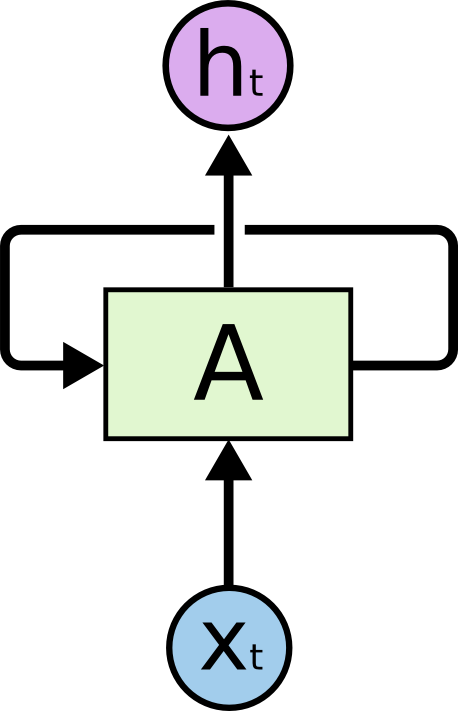
\includegraphics[width=0.30\textwidth]{pictures/RNN-rolled.png}
\caption[RNN Loop]{RNN loop\protect\footnotemark}
%%\end{floatingfigure} 
\end{figure}
\footnotetext{Quelle: "colah" \url{https://colah.github.io/posts/2015-08-Understanding-LSTMs/}}
In the above diagram, a chunk of neural network, A, looks at some input xt and outputs a value ht. A loop allows information to be passed from one step of the network to the next.

These loops make recurrent neural networks seem kind of mysterious. However, if you think a bit more, it turns out that they aren’t all that different than a normal neural network. A recurrent neural network can be thought of as multiple copies of the same network, each passing a message to a successor. Consider what happens if we unroll the loop:
\renewcommand{\figurename}{Abb.}
\begin{figure}[htp]
%%\begin{floatingfigure}[r]{textwidth}
\centering
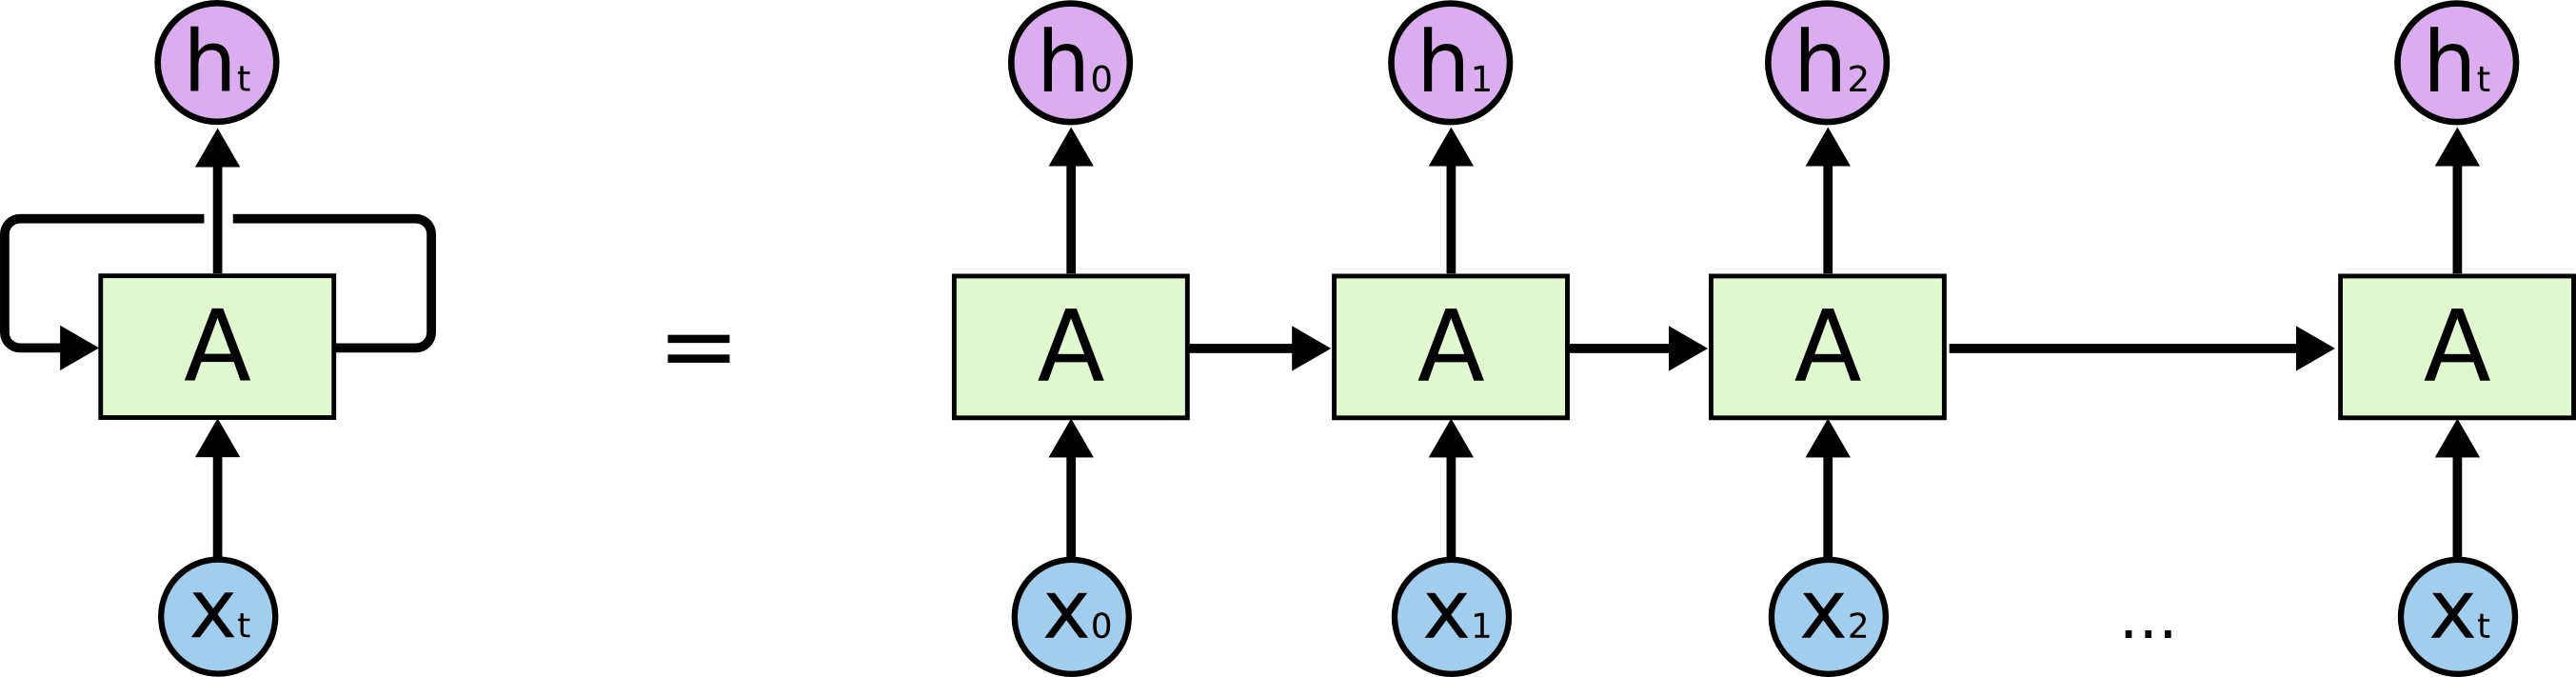
\includegraphics[width=0.60\textwidth]{pictures/RNN-unrolled.png}
\caption[unrolled RNN]{unrolled RNN\protect\footnotemark}
%%\end{floatingfigure} 
\end{figure}
\footnotetext{Quelle:  "colah" \url{https://colah.github.io/posts/2015-08-Understanding-LSTMs/}}
This chain-like nature reveals that recurrent neural networks are intimately related to sequences and lists. They’re the natural architecture of neural network to use for such data.

And they certainly are used! In the last few years, there have been incredible success applying RNNs to a variety of problems: speech recognition, language modeling, translation, image captioning… The list goes on. I’ll leave discussion of the amazing feats one can achieve with RNNs to Andrej Karpathy’s excellent blog post, The Unreasonable Effectiveness of Recurrent Neural Networks. But they really are pretty amazing.

Essential to these successes is the use of "LSTMs," a very special kind of recurrent neural network which works, for many tasks, much much better than the standard version. Almost all exciting results based on recurrent neural networks are achieved with them. It’s these LSTMs that this essay will explore.


\subsection{Backpropagation Through Time (BPTT) (unfinished)}
http://deeplearning4j.org/lstm.html
Remember, the purpose of recurrent nets is to accurately classify sequential input. We rely on the backpropagation of error and gradient descent to do so.
Backpropagation in feedforward networks moves backward from the final error through the outputs, weights and inputs of each hidden layer, assigning those weights responsibility for a portion of the error by calculating their partial derivatives – ∂E/∂w, or the relationship between their rates of change. Those derivatives are then used by our learning rule, gradient descent, to adjust the weights up or down, whichever direction decreases error.

Recurrent networks rely on an extension of backpropagation called backpropagation through time, or BPTT. Time, in this case, is simply expressed by a well-defined, ordered series of calculations linking one time step to the next, which is all backpropagation needs to work.

Neural networks, whether they are recurrent or not, are simply nested composite functions like f(g(h(x))). Adding a time element only extends the series of functions for which we calculate derivatives with the chain rule.

Truncated BPTT

Truncated BPTT is an approximation of full BPTT that is preferred for long sequences, since full BPTT’s forward/backward cost per parameter update becomes very high over many time steps. The downside is that the gradient can only flow back so far due to that truncation, so the network can’t learn dependencies that are as long as in full BPTT.

\subsection{Vanishing (and Exploding) Gradients (unfinished)}
http://deeplearning4j.org/lstm.html
Like most neural networks, recurrent nets are old. By the early 1990s, the vanishing gradient problem emerged as a major obstacle to recurrent net performance.

Just as a straight line expresses a change in x alongside a change in y, the gradient expresses the change in all weights with regard to the change in error. If we can’t know the gradient, we can’t adjust the weights in a direction that will decrease error, and our network ceases to learn.

Recurrent nets seeking to establish connections between a final output and events many time steps before were hobbled, because it is very difficult to know how much importance to accord to remote inputs. (Like great-great-*-grandparents, they multiply quickly in number and their legacy is often obscure.)

This is partially because the information flowing through neural nets passes through many stages of multiplication.

Everyone who has studied compound interest knows that any quantity multiplied frequently by an amount slightly greater than one can become immeasurably large (indeed, that simple mathematical truth underpins network effects and inevitable social inequalities). But its inverse, multiplying by a quantity less than one, is also true. Gamblers go bankrupt fast when they win just 97 cents on every dollar they put in the slots.

Because the layers and time steps of deep neural networks relate to each other through multiplication, derivatives are susceptible to vanishing or exploding.

Exploding gradients treat every weight as though it were the proverbial butterfly whose flapping wings cause a distant hurricane. Those weights’ gradients become saturated on the high end; i.e. they are presumed to be too powerful. But exploding gradients can be solved relatively easily, because they can be truncated or squashed. Vanishing gradients can become too small for computers to work with or for networks to learn – a harder problem to solve.

Below you see the effects of applying a sigmoid function over and over again. The data is flattened until, for large stretches, it has no detectable slope. This is analogous to a gradient vanishing as it passes through many layers.

\renewcommand{\figurename}{Abb.}
\begin{figure}[htp]
%%\begin{floatingfigure}[r]{textwidth}
\centering
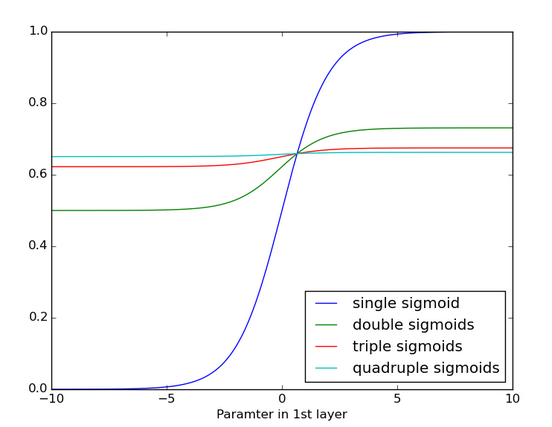
\includegraphics[width=0.60\textwidth]{pictures/sigmoid_vanishing_gradient.png}
\caption[Sigmoid Funktion]{Vanishing Gradient anhand von sigmoid function verdeutlicht\protect\footnotemark}
%%\end{floatingfigure} 
\end{figure}
\footnotetext{Quelle:  DL4J \url{http://deeplearning4j.org/lstm.htm}}

\subsection{The problem of long-term dependencies (unfinished)}
One of the appeals of RNNs is the idea that they might be able to connect previous information to the present task, such as using previous video frames might inform the understanding of the present frame. If RNNs could do this, they’d be extremely useful. But can they? It depends.

Sometimes, we only need to look at recent information to perform the present task. For example, consider a language model trying to predict the next word based on the previous ones. If we are trying to predict the last word in "the clouds are in the sky," we don’t need any further context – it’s pretty obvious the next word is going to be sky. In such cases, where the gap between the relevant information and the place that it’s needed is small, RNNs can learn to use the past information.
\renewcommand{\figurename}{Abb.}
\begin{figure}[htp]
%%\begin{floatingfigure}[r]{textwidth}
\centering
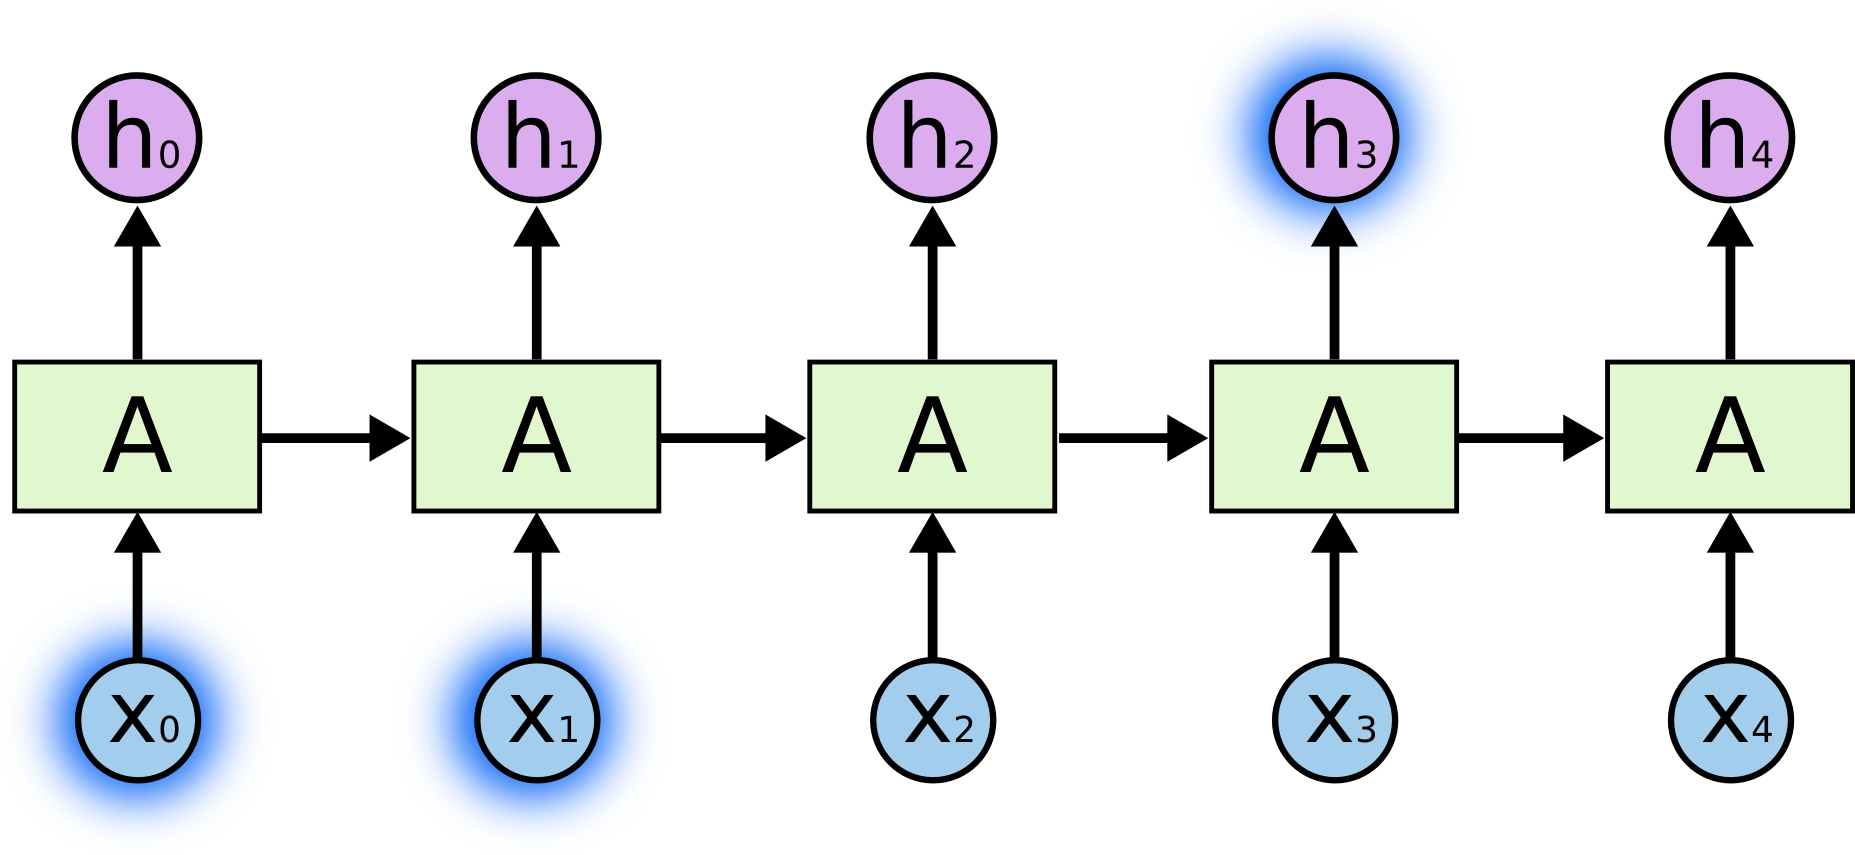
\includegraphics[width=0.60\textwidth]{pictures/RNN-shorttermdepdencies.png}
\caption[RNN short term dependencies]{RNN short term dependencies\protect\footnotemark}
%%\end{floatingfigure} 
\end{figure}
\footnotetext{Quelle:  "colah" \url{https://colah.github.io/posts/2015-08-Understanding-LSTMs/}}
But there are also cases where we need more context. Consider trying to predict the last word in the text "I grew up in France… I speak fluent French." Recent information suggests that the next word is probably the name of a language, but if we want to narrow down which language, we need the context of France, from further back. It’s entirely possible for the gap between the relevant information and the point where it is needed to become very large.

Unfortunately, as that gap grows, RNNs become unable to learn to connect the information.
\renewcommand{\figurename}{Abb.}
\begin{figure}[htp]
%%\begin{floatingfigure}[r]{textwidth}
\centering
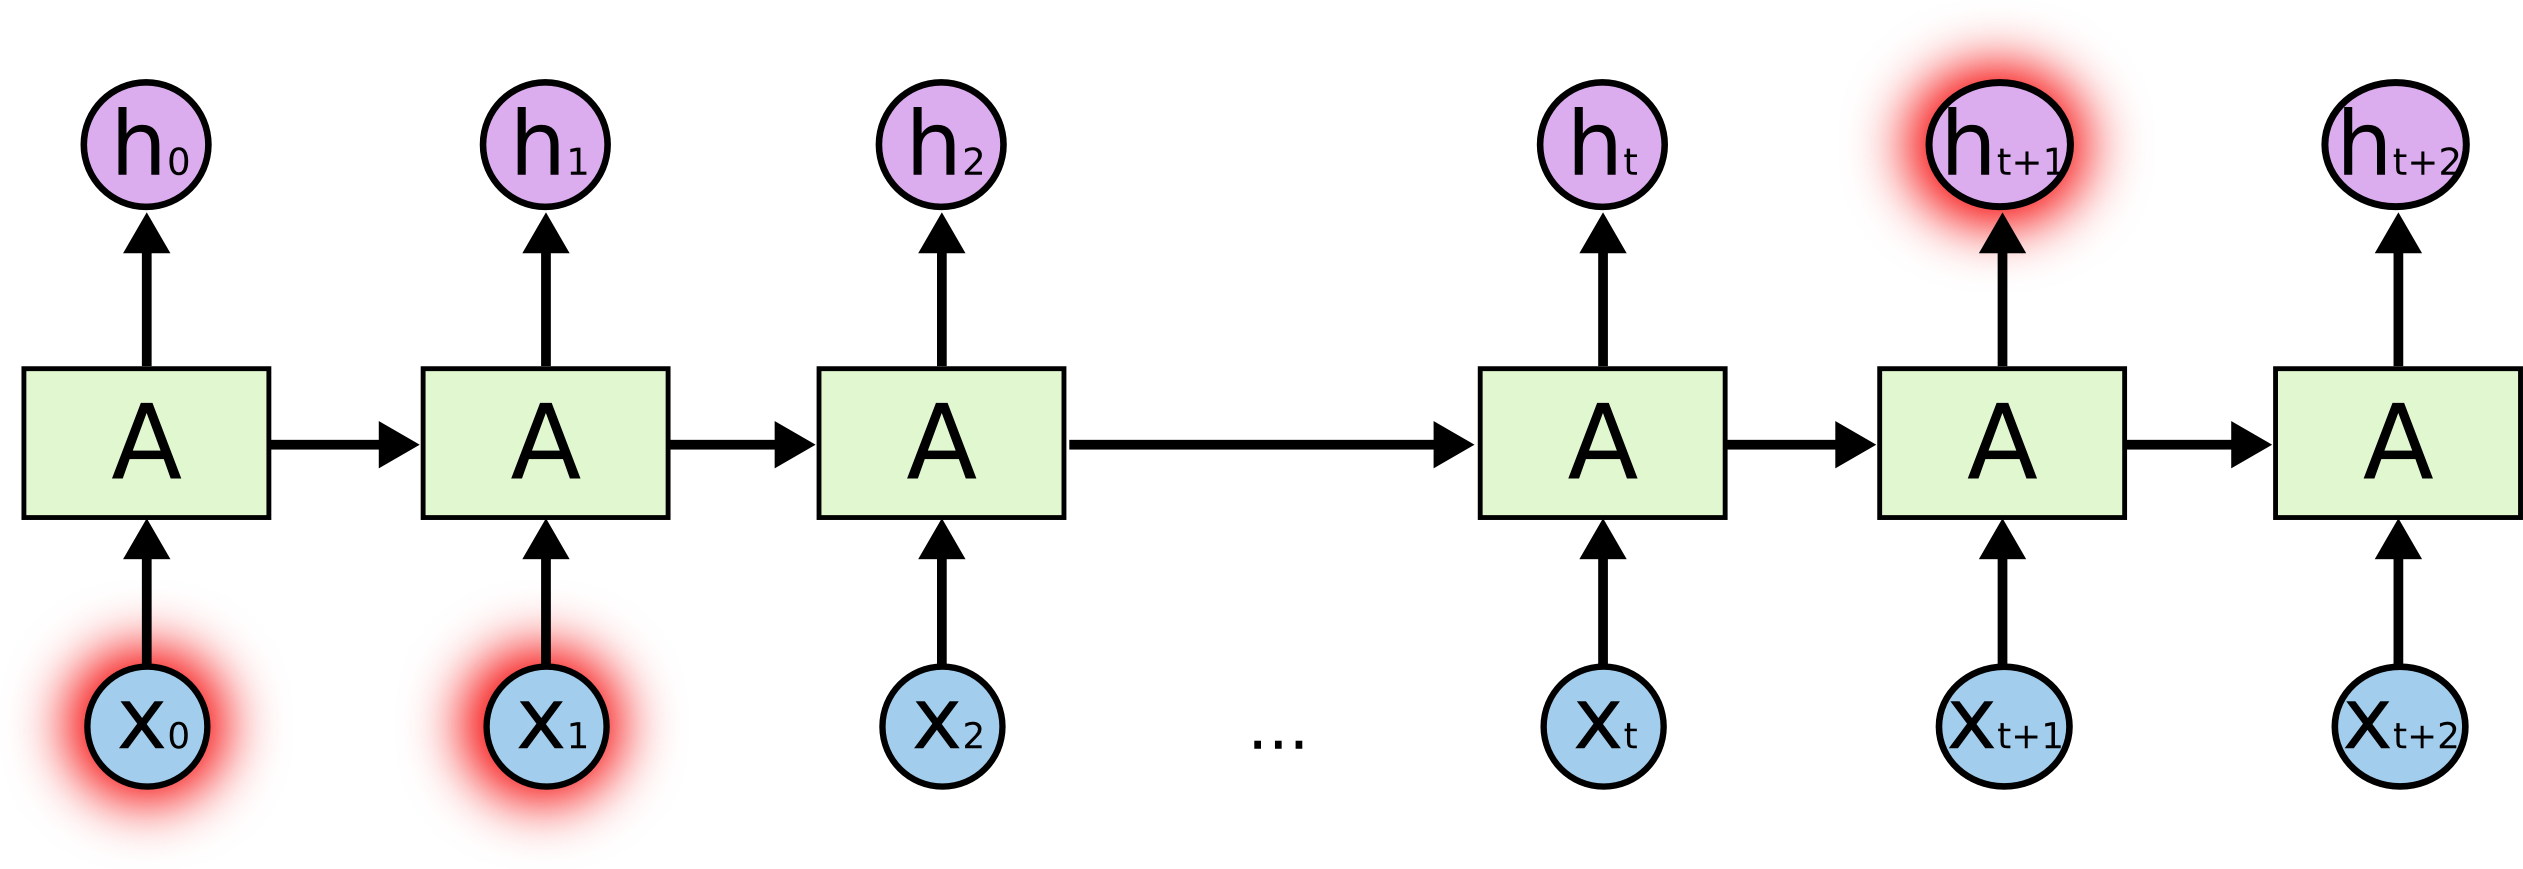
\includegraphics[width=0.60\textwidth]{pictures/RNN-longtermdependencies.png}
\caption[RNN long term dependencies]{RNN long term dependencies\protect\footnotemark}
%%\end{floatingfigure} 
\end{figure}
\footnotetext{Quelle:  "colah" \url{https://colah.github.io/posts/2015-08-Understanding-LSTMs/}}
In theory, RNNs are absolutely capable of handling such "long-term dependencies." A human could carefully pick parameters for them to solve toy problems of this form. Sadly, in practice, RNNs don’t seem to be able to learn them. The problem was explored in depth by Hochreiter (1991) [German] and Bengio, et al. (1994), who found some pretty fundamental reasons why it might be difficult.

Thankfully, LSTMs don’t have this problem!


\section{Long Short-Term Memory (LSTM) (unfinished)}
http://deeplearning4j.org/lstm.html
In the mid-90s, a variation of recurrent net with so-called Long Short-Term Memory units, or LSTMs, was proposed by the German researchers Sepp Hochreiter and Juergen Schmidhuber as a solution to the vanishing gradient problem.

LSTMs help preserve the error that can be backpropagated through time and layers. By maintaining a more constant error, they allow recurrent nets to continue to learn over many time steps (over 1000), thereby opening a channel to link causes and effects remotely.

LSTMs contain information outside the normal flow of the recurrent network in a gated cell. Information can be stored in, written to, or read from a cell, much like data in a computer’s memory. The cell makes decisions about what to store, and when to allow reads, writes and erasures, via gates that open and close. Unlike the digital storage on computers, however, these gates are analog, implemented with element-wise multiplication by sigmoids, which are all in the range of 0-1. Analog has the advantage over digital of being differentiable, and therefore suitable for backpropagation.

Those gates act on the signals they receive, and similar to the neural network’s nodes, they block or pass on information based on its strength and import, which they filter with their own sets of weights. Those weights, like the weights that modulate input and hidden states, are adjusted via the recurrent networks learning process. That is, the cells learn when to allow data to enter, leave or be deleted through the iterative process of making guesses, backpropagating error, and adjusting weights via gradient descent.

The diagram below illustrates how data flows through a memory cell and is controlled by its gates.

\renewcommand{\figurename}{Abb.}
\begin{figure}[htp]
%%\begin{floatingfigure}[r]{textwidth}
\centering
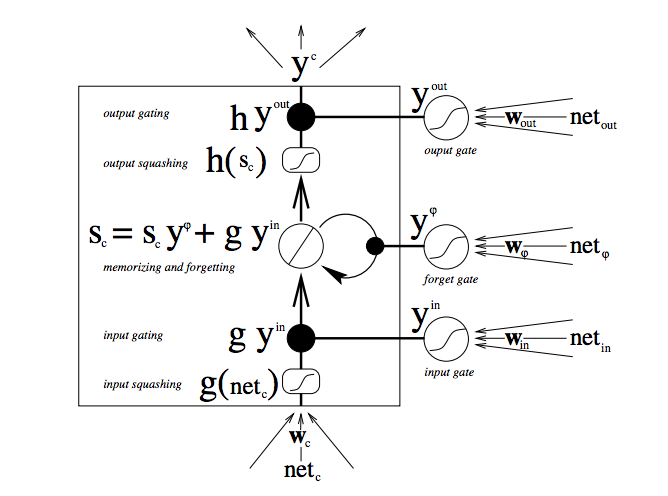
\includegraphics[width=0.60\textwidth]{pictures/gers_lstm.png}
\caption[Memory Cell]{Memory cell\protect\footnotemark}
%%\end{floatingfigure} 
\end{figure}
\footnotetext{Quelle:  DL4J \url{http://deeplearning4j.org/lstm.htm}}

Starting from the bottom, the triple arrows show where information flows into the cell at multiple points. That combination of present input and past cell state is fed not only to the cell itself, but also to each of its three gates, which will decide how the input will be handled.

The black dots are the gates themselves, which determine respectively whether to let new input in, erase the present cell state, and/or let that state impact the network’s output at the present time step. S\_c is the current state of the memory cell, and g\_y\_in is the current input to it. Remember that each gate can be open or shut, and they will recombine their open and shut states at each step. The cell can forget its state, or not; be written to, or not; and be read from, or not, at each time step, and those flows are represented here.

The large bold letters give us the result of each operation.

Here’s another diagram for good measure, comparing a simple recurrent network (left) to an LSTM cell (right). The blue lines can be ignored; the legend is helpful.

\renewcommand{\figurename}{Abb.}
\begin{figure}[htp]
%%\begin{floatingfigure}[r]{textwidth}
\centering
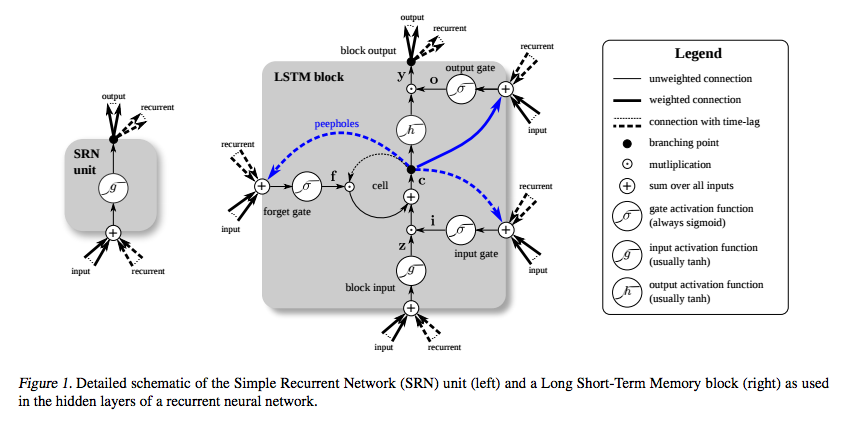
\includegraphics[width=0.60\textwidth]{pictures/greff_lstm_diagram.png}
\caption[Vergleich Recurrent Network und LSTM]{Vergleich: Simple Recurrent Network(SRN) und LSTM block\protect\footnotemark}
%%\end{floatingfigure} 
\end{figure}
\footnotetext{Quelle:  DL4J \url{http://deeplearning4j.org/lstm.htm}}

It’s important to note that LSTMs’ memory cells give different roles to addition and multiplication in the transformation of input. The central plus sign in both diagrams is essentially the secret of LSTMs. Stupidly simple as it may seem, this basic change helps them preserve a constant error when it must be backpropagated at depth. Instead of determining the subsequent cell state by multiplying its current state with new input, they add the two, and that quite literally makes the difference. (The forget gate still relies on multiplication, of course.)

Different sets of weights filter the input for input, output and forgetting. The forget gate is represented as a linear identity function, because if the gate is open, the current state of the memory cell is simply multiplied by one, to propagate forward one more time step.

Furthermore, while we’re on the topic of simple hacks, including a bias of 1 to the forget gate of every LSTM cell is also shown to improve performance.

You may wonder why LSTMs have a forget gate when their purpose is to link distant occurrences to a final output. Well, sometimes it’s good to forget. If you’re analyzing a text corpus and come to the end of a document, for example, you may have no reason to believe that the next document has any relationship to it whatsoever, and therefore the memory cell should be set to zero before the net ingests the first element of the next document.

In the diagram below, you can see the gates at work, with straight lines representing closed gates, and blank circles representing open ones. The lines and circles running horizontal down the hidden layer are the forget gates.

\renewcommand{\figurename}{Abb.}
\begin{figure}[htp]
%%\begin{floatingfigure}[r]{textwidth}
\centering
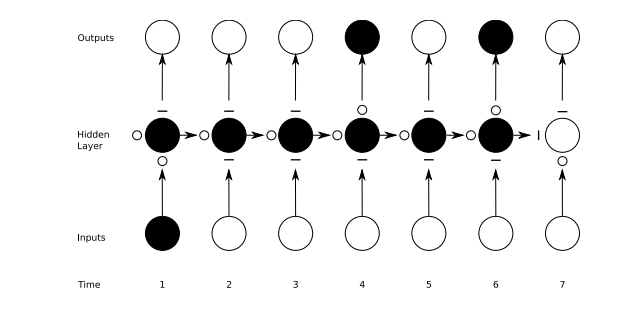
\includegraphics[width=0.60\textwidth]{pictures/gates_lstm.png}
\caption[Gates at work]{Gates at work\protect\footnotemark}
%%\end{floatingfigure} 
\end{figure}
\footnotetext{Quelle:  DL4J \url{http://deeplearning4j.org/lstm.htm}}

It should be noted that while feedforward networks map one input to one output, recurrent nets can map one to many, as above (one image to many words in a caption), many to many (translation), or many to one (classifying a voice).

"Capturing Diverse Time Scales and Remote Dependencies"

You may also wonder what the precise value is of input gates that protect a memory cell from new data coming in, and output gates that prevent it from affecting certain outputs of the RNN. You can think of LSTMs as allowing a neural network to operate on different scales of time at once.

Let’s take a human life, and imagine that we are receiving various streams of data about that life in a time series. Geolocation at each time step is pretty important for the next time step, so that scale of time is always open to the latest information.

Perhaps this human is a diligent citizen who votes every couple years. On democratic time, we would want to pay special attention to what they do around elections, before they return to making a living, and away from larger issues. We would not want to let the constant noise of geolocation affect our political analysis.

If this human is also a diligent daughter, then maybe we can construct a familial time that learns patterns in phone calls which take place regularly every Sunday and spike annually around the holidays. Little to do with political cycles or geolocation.

Other data is like that. Music is polyrhythmic. Text contains recurrent themes at varying intervals. Stock markets and economies experience jitters within longer waves. They operate simultaneously on different time scales that LSTMs can capture.

Further links: (could be sources for pictures)
http://people.idsia.ch/~juergen/rnn.html
https://karpathy.github.io/2015/05/21/rnn-effectiveness/
https://www.cs.cmu.edu/~bhiksha/courses/deeplearning/Fall.2015/pdfs/Werbos.backprop.pdf
http://www.cs.toronto.edu/~graves/phd.pdf
http://www.felixgers.de/papers/phd.pdf
http://arxiv.org/pdf/1503.04069.pdf


https://colah.github.io/posts/2015-08-Understanding-LSTMs/
Long Short Term Memory networks – usually just called "LSTMs" – are a special kind of RNN, capable of learning long-term dependencies. They were introduced by Hochreiter \& Schmidhuber (1997), and were refined and popularized by many people in following work.1 They work tremendously well on a large variety of problems, and are now widely used.

LSTMs are explicitly designed to avoid the long-term dependency problem. Remembering information for long periods of time is practically their default behavior, not something they struggle to learn!

All recurrent neural networks have the form of a chain of repeating modules of neural network. In standard RNNs, this repeating module will have a very simple structure, such as a single tanh layer.
\renewcommand{\figurename}{Abb.}
\begin{figure}[htp]
%%\begin{floatingfigure}[r]{textwidth}
\centering
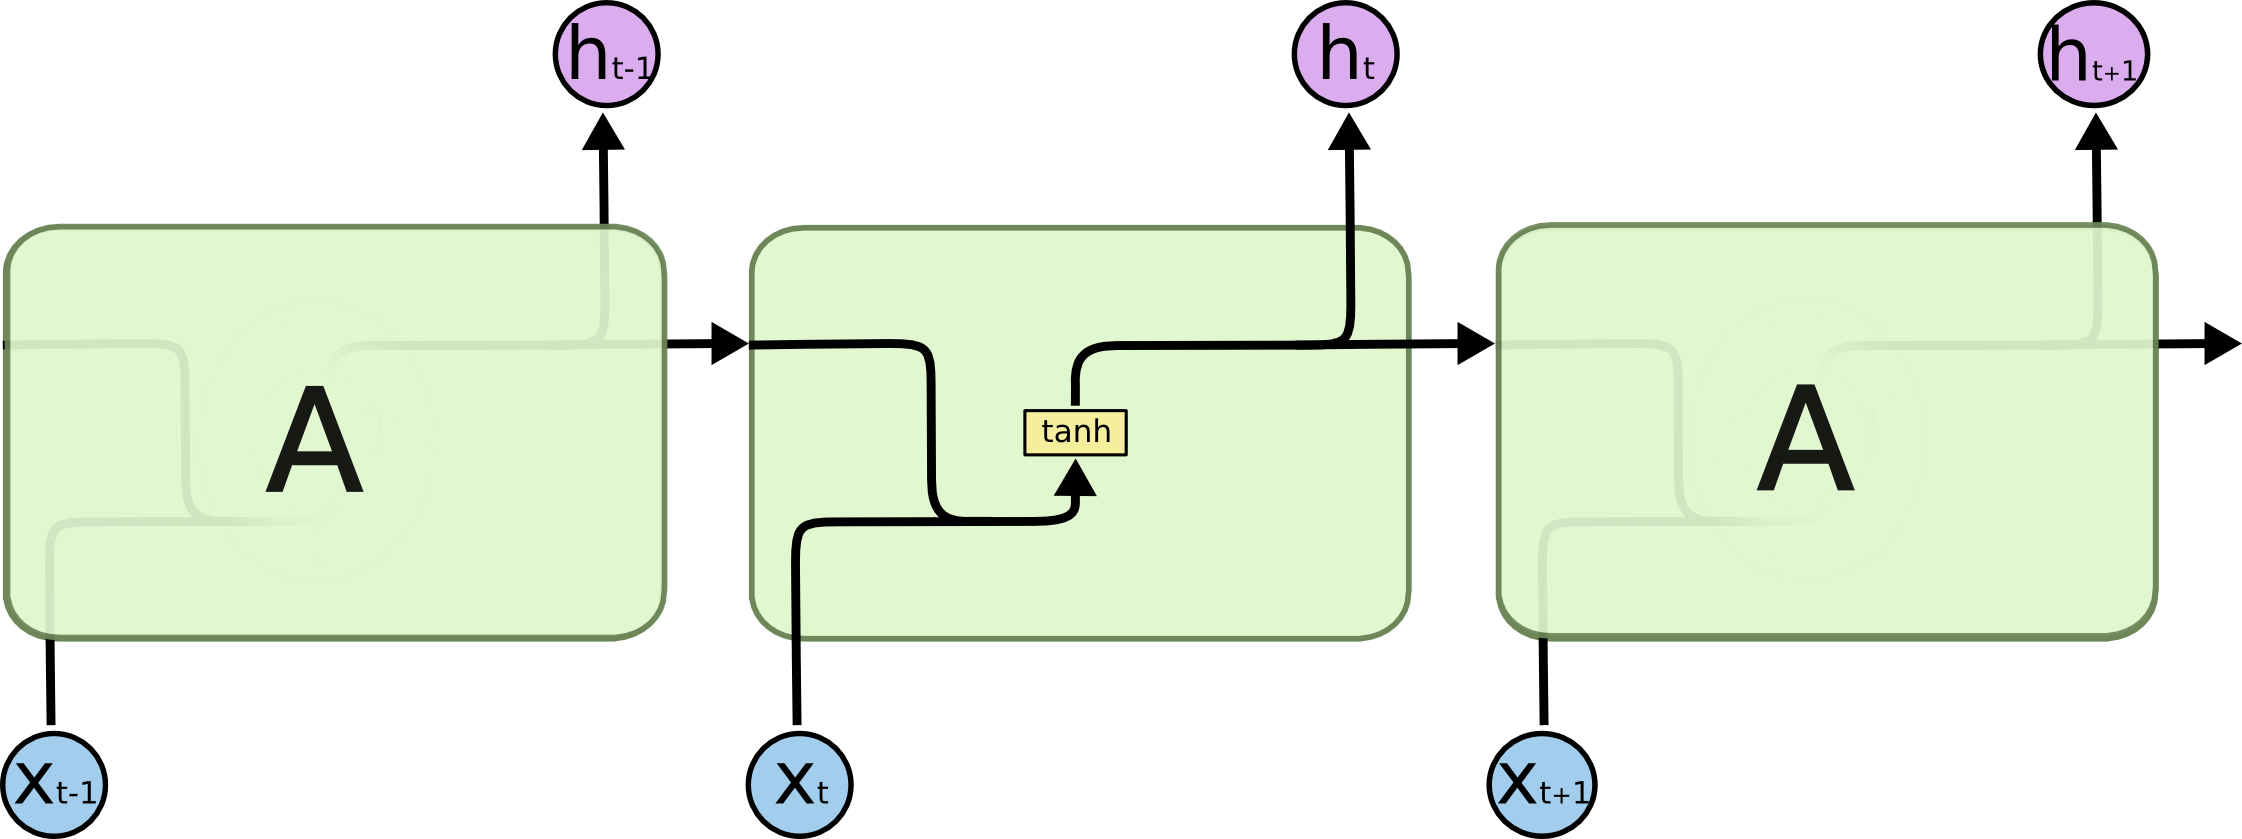
\includegraphics[width=0.60\textwidth]{pictures/LSTM3-SimpleRNN.png}
\caption[Repeating module of standard RNN]{The repeating module in a standard RNN contains a single layer.\protect\footnotemark}
%%\end{floatingfigure} 
\end{figure}
\footnotetext{Quelle:  "colah" \url{https://colah.github.io/posts/2015-08-Understanding-LSTMs/}}
LSTMs also have this chain like structure, but the repeating module has a different structure. Instead of having a single neural network layer, there are four, interacting in a very special way.
\renewcommand{\figurename}{Abb.}
\begin{figure}[htp]
%%\begin{floatingfigure}[r]{textwidth}
\centering
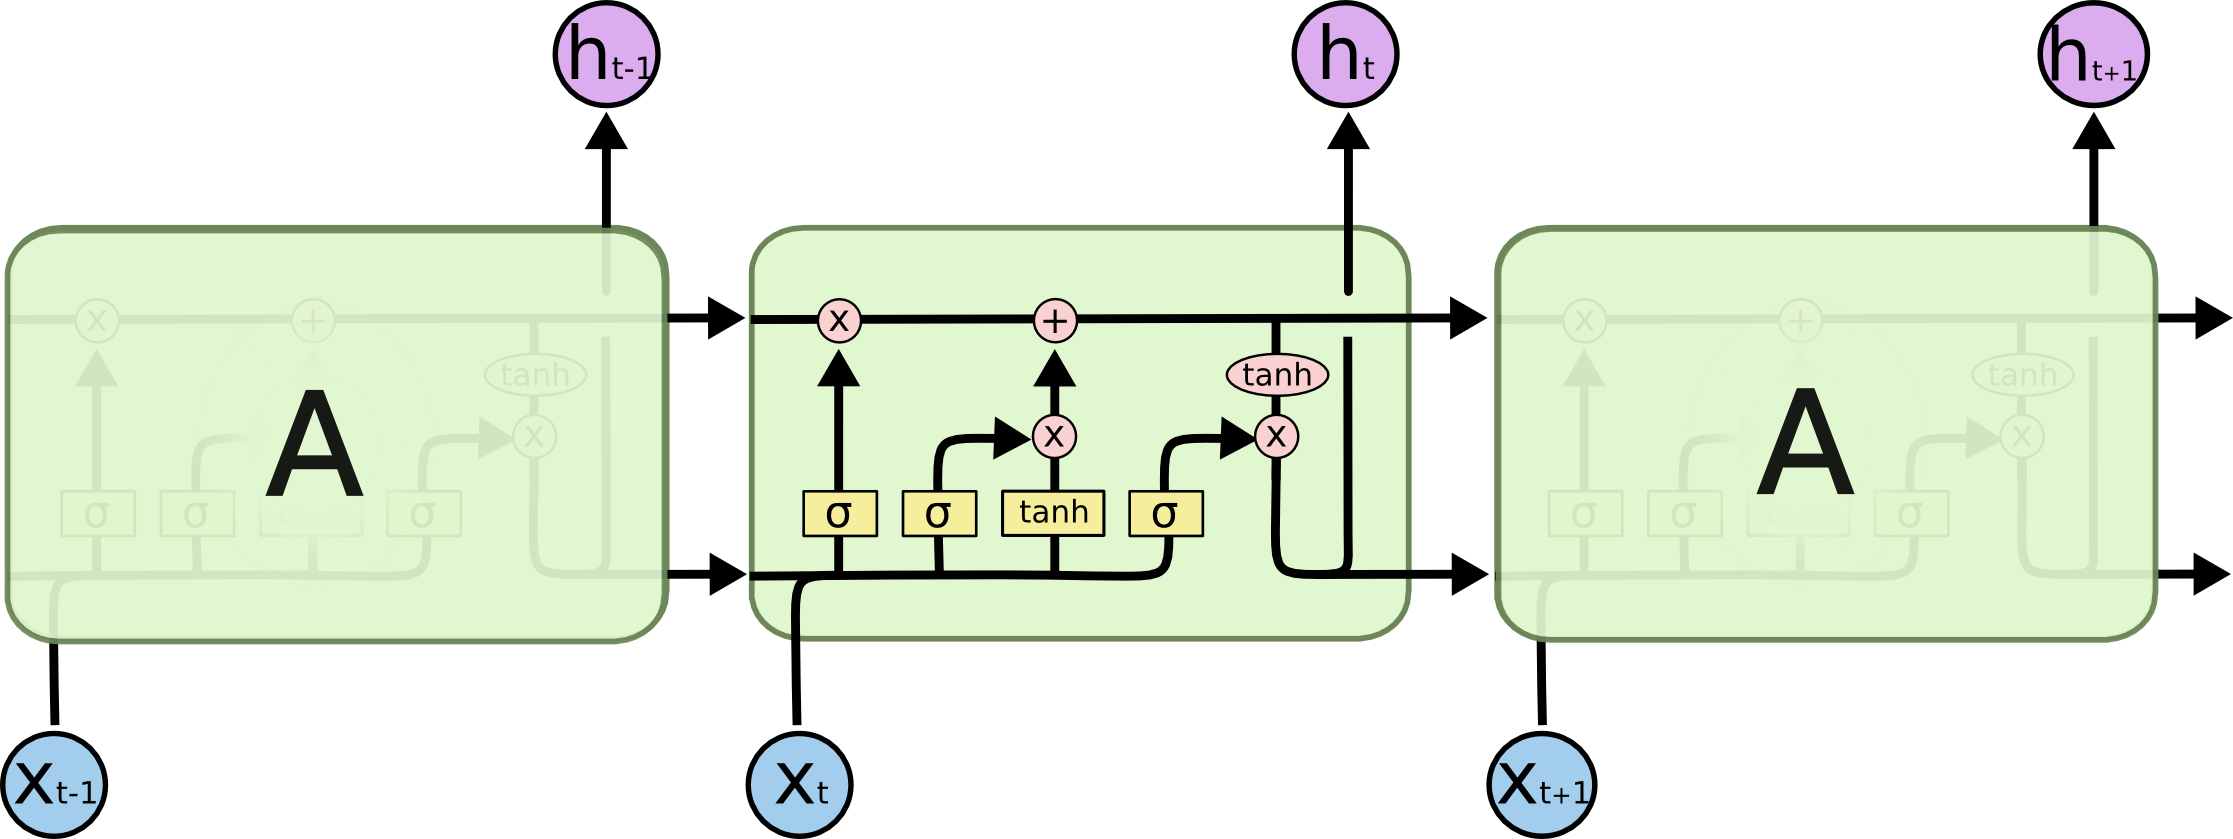
\includegraphics[width=0.60\textwidth]{pictures/LSTM3-chain.png}
\caption[Repeating module of LSTM]{The repeating module in an LSTM contains four interacting layers.\protect\footnotemark}
%%\end{floatingfigure} 
\end{figure}
\footnotetext{Quelle:  "colah" \url{https://colah.github.io/posts/2015-08-Understanding-LSTMs/}}
Don’t worry about the details of what’s going on. We’ll walk through the LSTM diagram step by step later. For now, let’s just try to get comfortable with the notation we’ll be using.
\renewcommand{\figurename}{Abb.}
\begin{figure}[htp]
%%\begin{floatingfigure}[r]{textwidth}
\centering
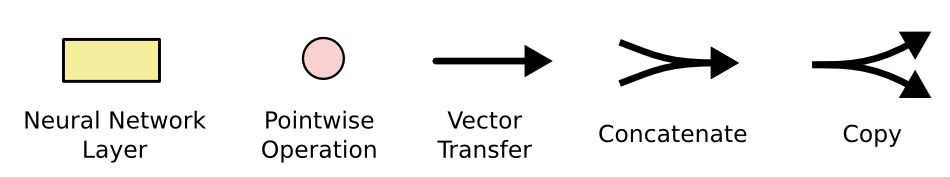
\includegraphics[width=0.60\textwidth]{pictures/LSTM2-notation.png}
\caption[LSTM anotation]{used notation\protect\footnotemark}
%%\end{floatingfigure} 
\end{figure}
\footnotetext{Quelle:  "colah" \url{https://colah.github.io/posts/2015-08-Understanding-LSTMs/}}
In the above diagram, each line carries an entire vector, from the output of one node to the inputs of others. The pink circles represent pointwise operations, like vector addition, while the yellow boxes are learned neural network layers. Lines merging denote concatenation, while a line forking denote its content being copied and the copies going to different locations. 

\subsubsection{The Core Idea Behind LSTMs}

The key to LSTMs is the cell state, the horizontal line running through the top of the diagram.
The cell state is kind of like a conveyor belt. It runs straight down the entire chain, with only some minor linear interactions. It’s very easy for information to just flow along it unchanged.
\renewcommand{\figurename}{Abb.}
\begin{figure}[htp]
%%\begin{floatingfigure}[r]{textwidth}
\centering
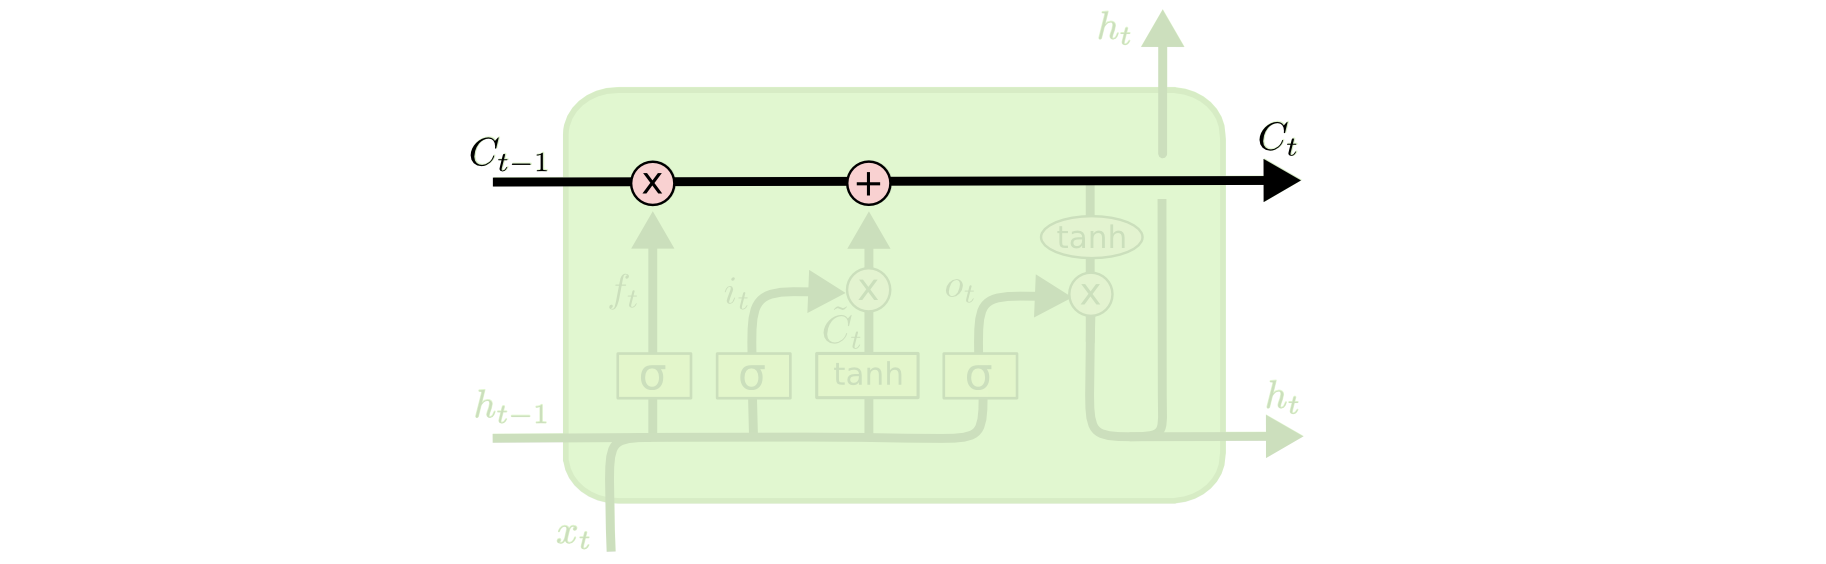
\includegraphics[width=0.60\textwidth]{pictures/LSTM3-C-line.png}
\caption[LSTM C line]{LSTM C line\protect\footnotemark}
%%\end{floatingfigure} 
\end{figure}
\footnotetext{Quelle:  "colah" \url{https://colah.github.io/posts/2015-08-Understanding-LSTMs/}}
The LSTM does have the ability to remove or add information to the cell state, carefully regulated by structures called gates.

Gates are a way to optionally let information through. They are composed out of a sigmoid neural net layer and a pointwise multiplication operation.
\renewcommand{\figurename}{Abb.}
\begin{figure}[htp]
%%\begin{floatingfigure}[r]{textwidth}
\centering
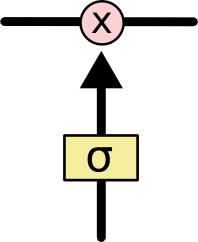
\includegraphics[width=0.30\textwidth]{pictures/LSTM3-gate.png}
\caption[LSTM gate]{LSTM gate\protect\footnotemark}
%%\end{floatingfigure} 
\end{figure}
\footnotetext{Quelle:  "colah" \url{https://colah.github.io/posts/2015-08-Understanding-LSTMs/}}
The sigmoid layer outputs numbers between zero and one, describing how much of each component should be let through. A value of zero means "let nothing through," while a value of one means "let everything through!"

An LSTM has three of these gates, to protect and control the cell state.

\subsubsection{Step-by-Step LSTM walk through}
The first step in our LSTM is to decide what information we’re going to throw away from the cell state. This decision is made by a sigmoid layer called the "forget gate layer." It looks at ht−1 and xt, and outputs a number between 0 and 1 for each number in the cell state Ct−1. A 1 represents "completely keep this" while a 0 represents "completely get rid of this."

Let’s go back to our example of a language model trying to predict the next word based on all the previous ones. In such a problem, the cell state might include the gender of the present subject, so that the correct pronouns can be used. When we see a new subject, we want to forget the gender of the old subject.
\renewcommand{\figurename}{Abb.}
\begin{figure}[htp]
%%\begin{floatingfigure}[r]{textwidth}
\centering
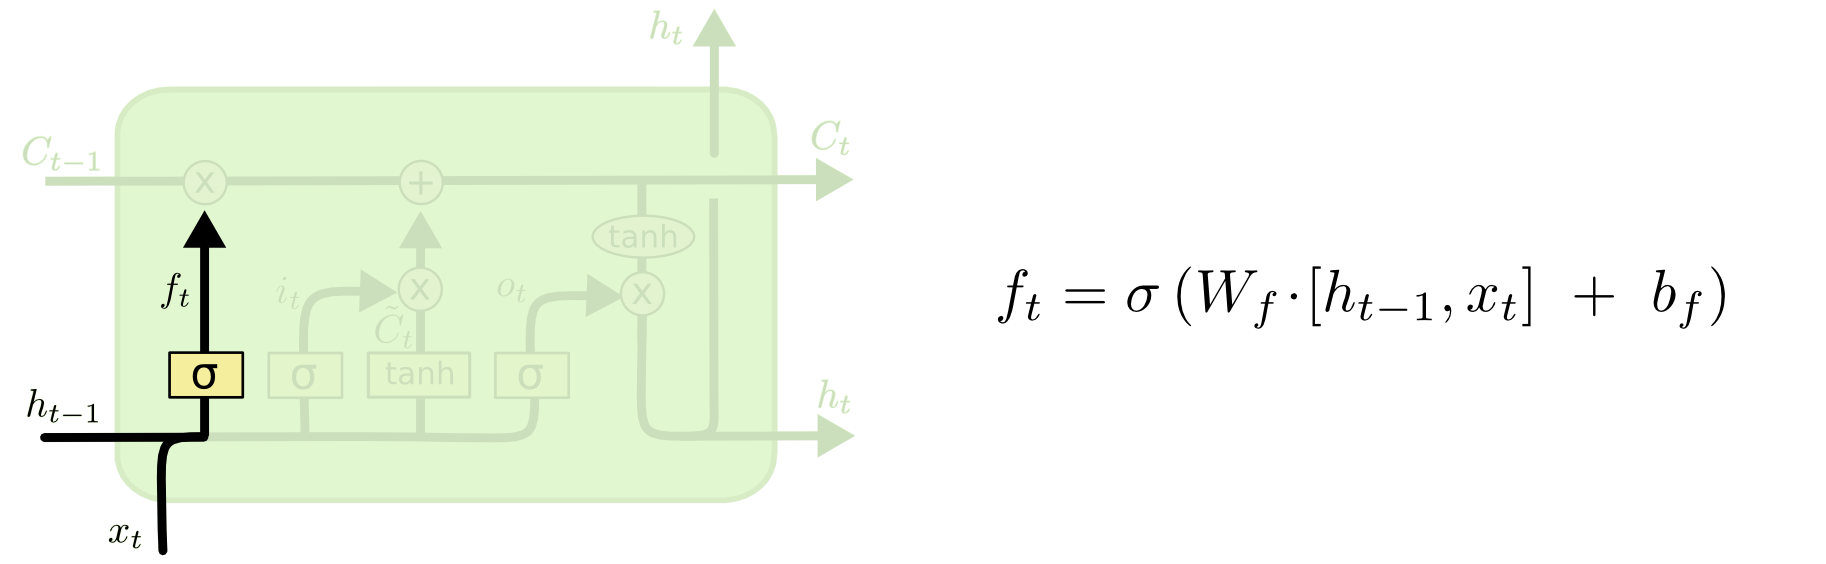
\includegraphics[width=0.60\textwidth]{pictures/LSTM3-focus-f.png}
\caption[LSTM focus f]{LSTM focus f\protect\footnotemark}
%%\end{floatingfigure} 
\end{figure}
\footnotetext{Quelle:  "colah" \url{https://colah.github.io/posts/2015-08-Understanding-LSTMs/}}
The next step is to decide what new information we’re going to store in the cell state. This has two parts. First, a sigmoid layer called the "input gate layer" decides which values we’ll update. Next, a tanh layer creates a vector of new candidate values, C~t, that could be added to the state. In the next step, we’ll combine these two to create an update to the state.

In the example of our language model, we’d want to add the gender of the new subject to the cell state, to replace the old one we’re forgetting.
\renewcommand{\figurename}{Abb.}
\begin{figure}[htp]
%%\begin{floatingfigure}[r]{textwidth}
\centering
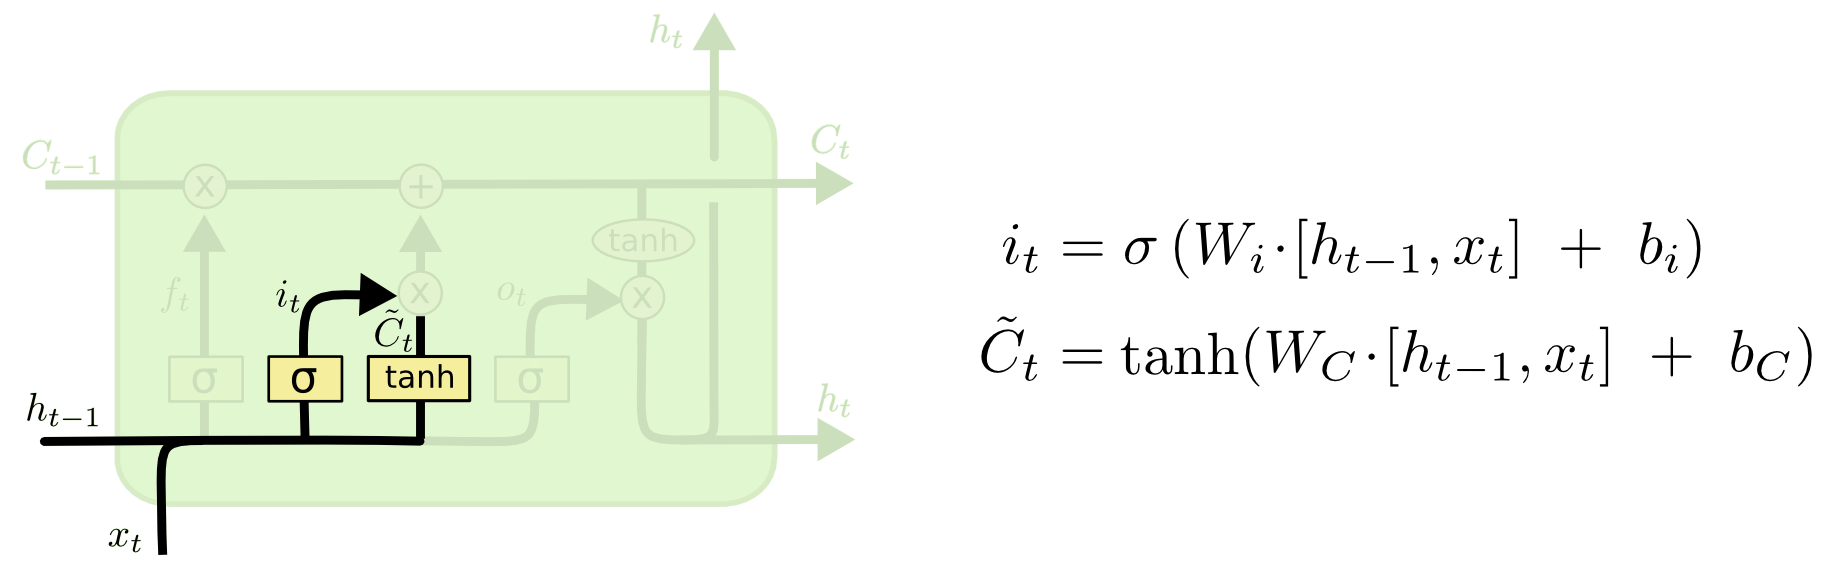
\includegraphics[width=0.60\textwidth]{pictures/LSTM3-focus-i.png}
\caption[LSTM focus i]{LSTM focus i\protect\footnotemark}
%%\end{floatingfigure} 
\end{figure}
\footnotetext{Quelle:  "colah" \url{https://colah.github.io/posts/2015-08-Understanding-LSTMs/}}
It’s now time to update the old cell state, Ct−1, into the new cell state Ct. The previous steps already decided what to do, we just need to actually do it.

We multiply the old state by ft, forgetting the things we decided to forget earlier. Then we add it∗C~t. This is the new candidate values, scaled by how much we decided to update each state value.

In the case of the language model, this is where we’d actually drop the information about the old subject’s gender and add the new information, as we decided in the previous steps.
\renewcommand{\figurename}{Abb.}
\begin{figure}[htp]
%%\begin{floatingfigure}[r]{textwidth}
\centering
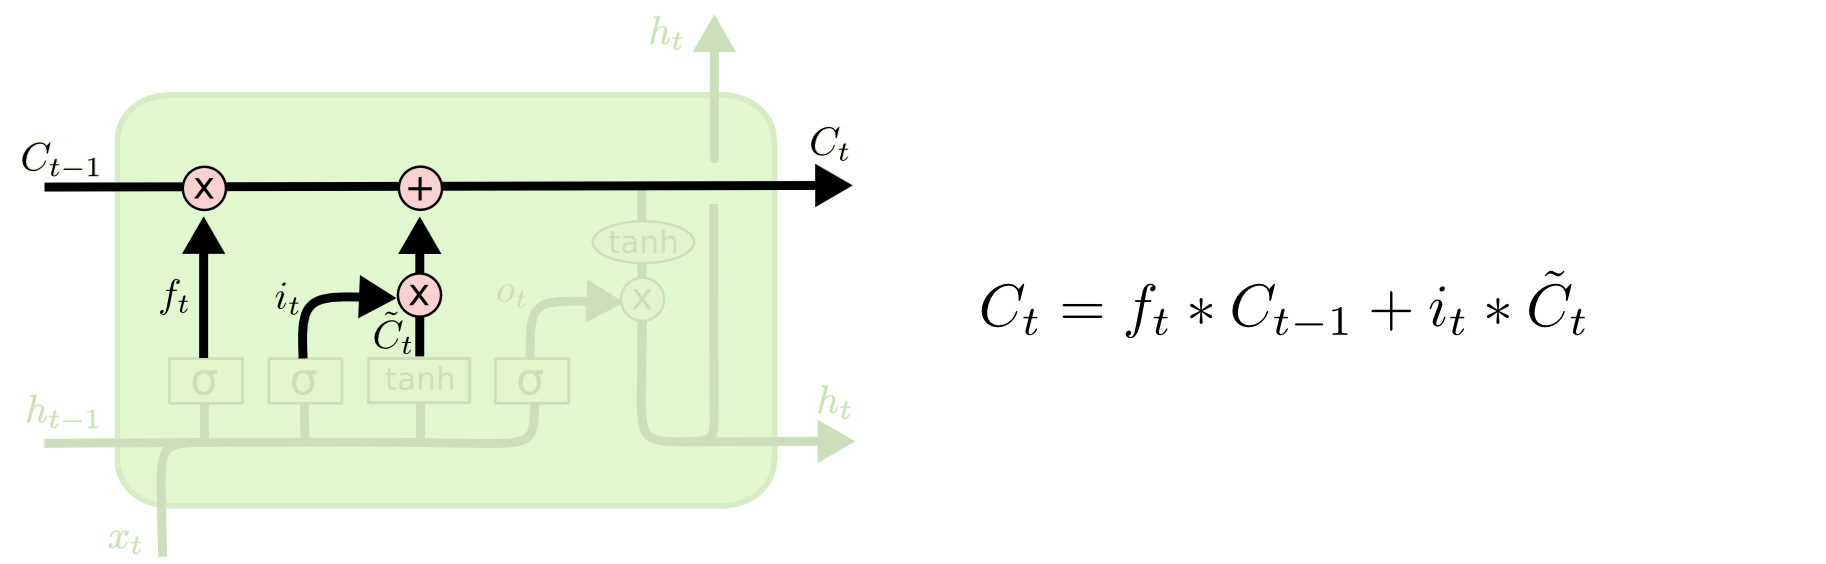
\includegraphics[width=0.60\textwidth]{pictures/LSTM3-focus-C.png}
\caption[LSTM focus C]{LSTM focus C\protect\footnotemark}
%%\end{floatingfigure} 
\end{figure}
\footnotetext{Quelle:  "colah" \url{https://colah.github.io/posts/2015-08-Understanding-LSTMs/}}
Finally, we need to decide what we’re going to output. This output will be based on our cell state, but will be a filtered version. First, we run a sigmoid layer which decides what parts of the cell state we’re going to output. Then, we put the cell state through tanh (to push the values to be between −1 and 1) and multiply it by the output of the sigmoid gate, so that we only output the parts we decided to.

For the language model example, since it just saw a subject, it might want to output information relevant to a verb, in case that’s what is coming next. For example, it might output whether the subject is singular or plural, so that we know what form a verb should be conjugated into if that’s what follows next.
\renewcommand{\figurename}{Abb.}
\begin{figure}[htp]
%%\begin{floatingfigure}[r]{textwidth}
\centering
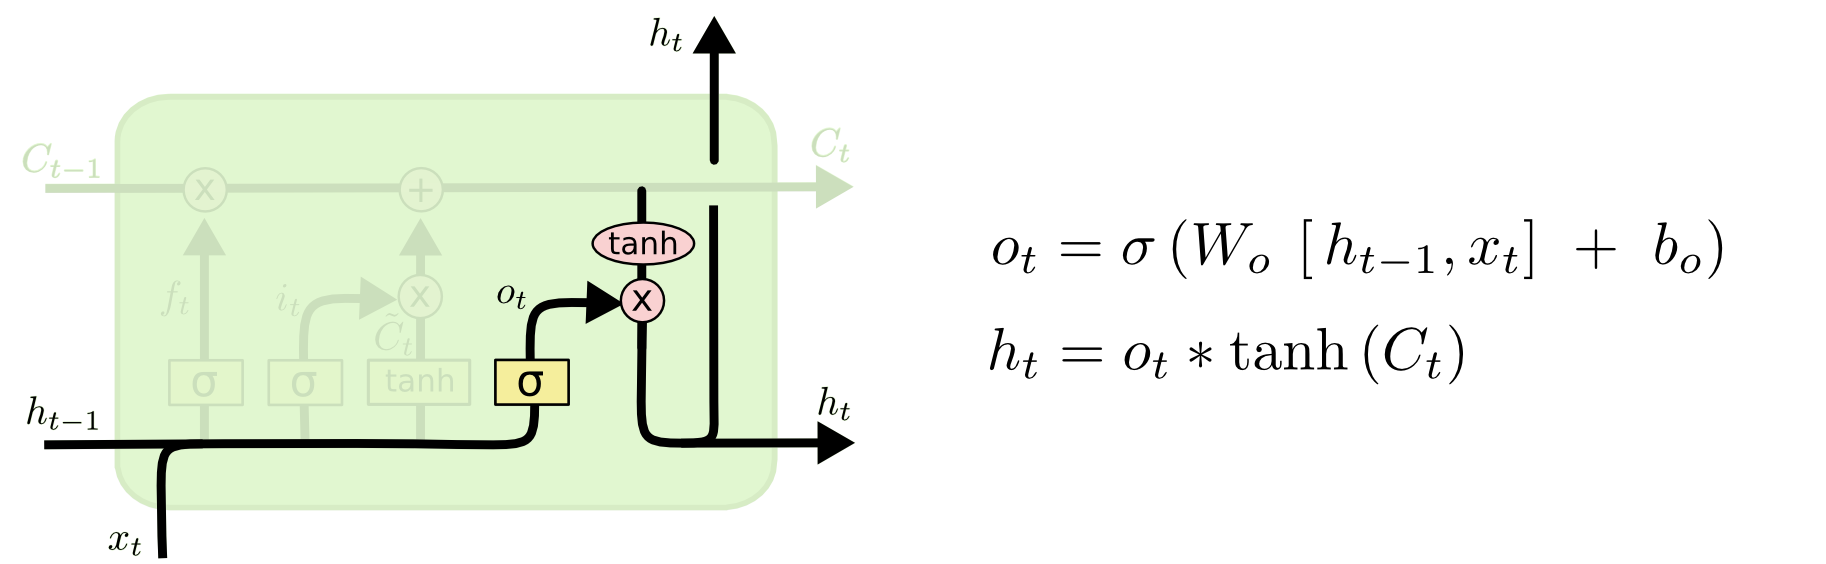
\includegraphics[width=0.60\textwidth]{pictures/LSTM3-focus-o.png}
\caption[LSTM focus o]{LSTM focus o\protect\footnotemark}
%%\end{floatingfigure} 
\end{figure}
\footnotetext{Quelle:  "colah" \url{https://colah.github.io/posts/2015-08-Understanding-LSTMs/}}

\subsubsection{Variants on Long Short Term Memory}
What I’ve described so far is a pretty normal LSTM. But not all LSTMs are the same as the above. In fact, it seems like almost every paper involving LSTMs uses a slightly different version. The differences are minor, but it’s worth mentioning some of them.

One popular LSTM variant, introduced by Gers \& Schmidhuber (2000), is adding "peephole connections." This means that we let the gate layers look at the cell state.
\renewcommand{\figurename}{Abb.}
\begin{figure}[htp]
%%\begin{floatingfigure}[r]{textwidth}
\centering
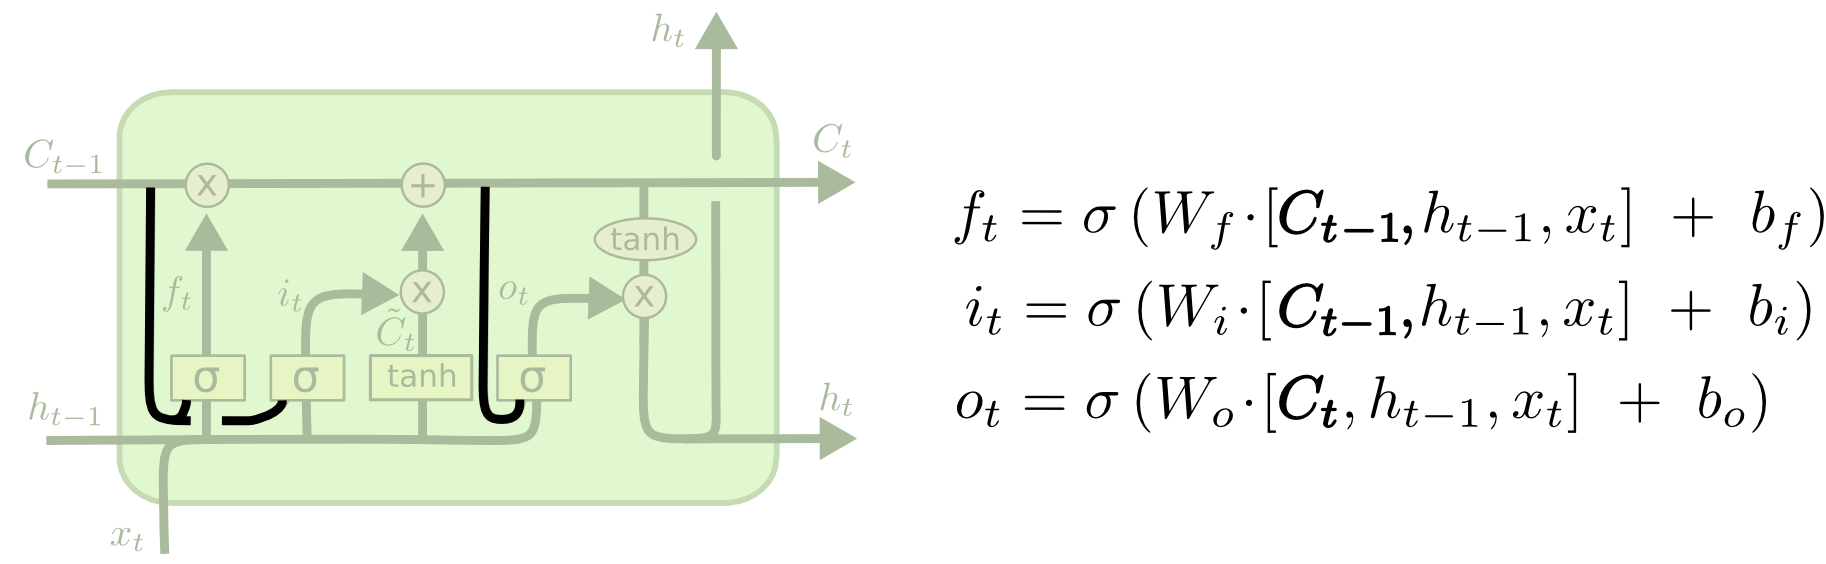
\includegraphics[width=0.60\textwidth]{pictures/LSTM3-var-peepholes.png}
\caption[LSTM peepholes]{LSTM peepholes\protect\footnotemark}
%%\end{floatingfigure} 
\end{figure}
\footnotetext{Quelle:  "colah" \url{https://colah.github.io/posts/2015-08-Understanding-LSTMs/}}
The above diagram adds peepholes to all the gates, but many papers will give some peepholes and not others.

Another variation is to use coupled forget and input gates. Instead of separately deciding what to forget and what we should add new information to, we make those decisions together. We only forget when we’re going to input something in its place. We only input new values to the state when we forget something older.
\renewcommand{\figurename}{Abb.}
\begin{figure}[htp]
%%\begin{floatingfigure}[r]{textwidth}
\centering
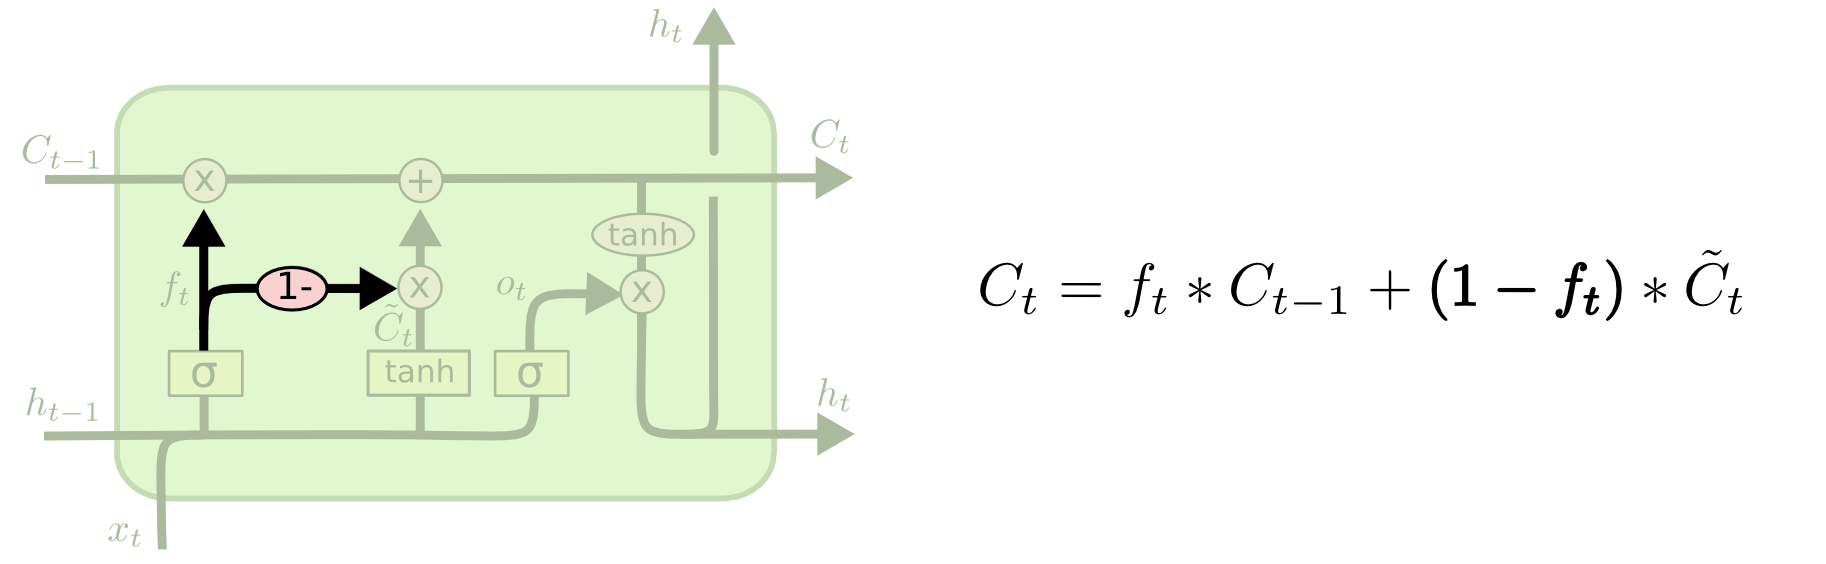
\includegraphics[width=0.60\textwidth]{pictures/LSTM3-var-tied.png}
\caption[LSTM tied]{LSTM tied\protect\footnotemark}
%%\end{floatingfigure} 
\end{figure}
\footnotetext{Quelle:  "colah" \url{https://colah.github.io/posts/2015-08-Understanding-LSTMs/}}
A slightly more dramatic variation on the LSTM is the Gated Recurrent Unit, or GRU, introduced by Cho, et al. (2014). It combines the forget and input gates into a single "update gate." It also merges the cell state and hidden state, and makes some other changes. The resulting model is simpler than standard LSTM models, and has been growing increasingly popular.
\renewcommand{\figurename}{Abb.}
\begin{figure}[htp]
%%\begin{floatingfigure}[r]{textwidth}
\centering
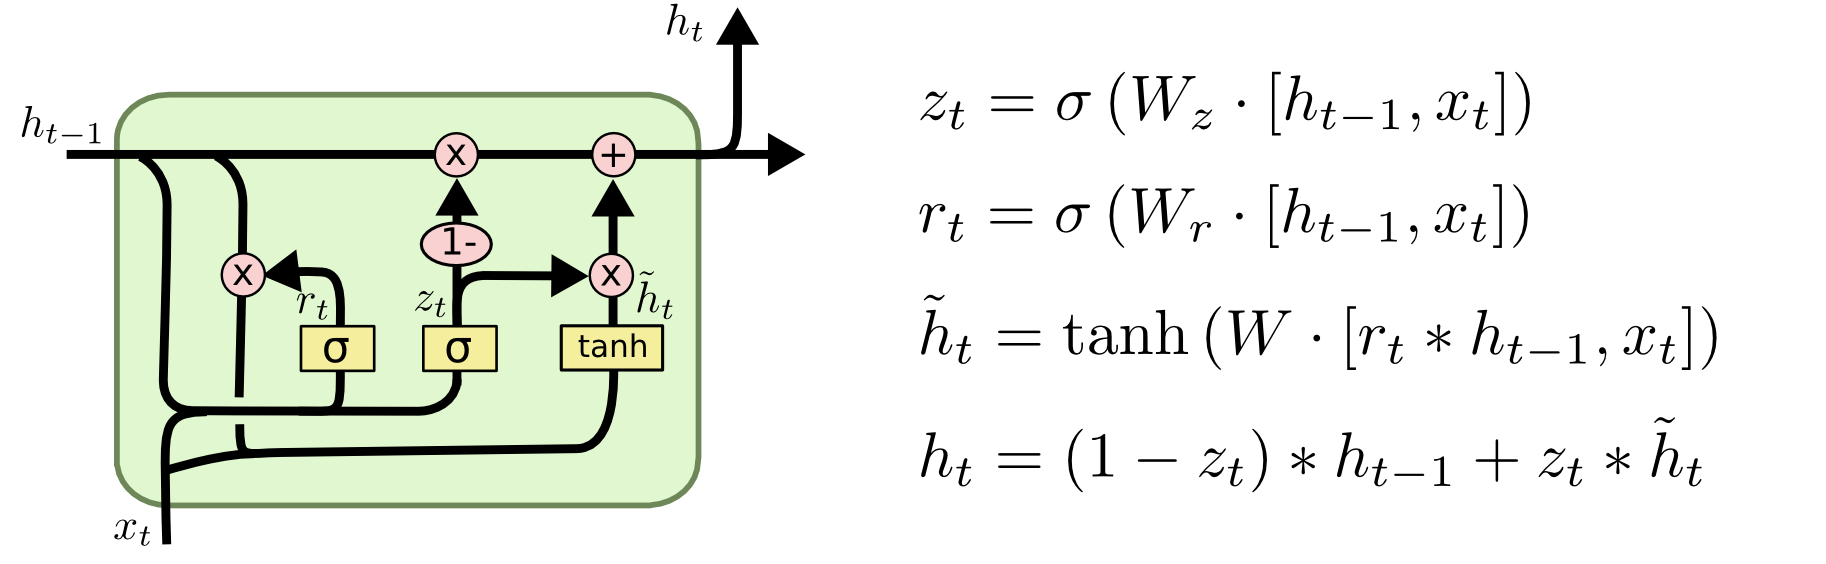
\includegraphics[width=0.60\textwidth]{pictures/LSTM3-var-GRU.png}
\caption[LSTM GRU]{LSTM GRU\protect\footnotemark}
%%\end{floatingfigure} 
\end{figure}
\footnotetext{Quelle:  "colah" \url{https://colah.github.io/posts/2015-08-Understanding-LSTMs/}}
These are only a few of the most notable LSTM variants. There are lots of others, like Depth Gated RNNs by Yao, et al. (2015). There’s also some completely different approach to tackling long-term dependencies, like Clockwork RNNs by Koutnik, et al. (2014).

Which of these variants is best? Do the differences matter? Greff, et al. (2015) do a nice comparison of popular variants, finding that they’re all about the same. Jozefowicz, et al. (2015) tested more than ten thousand RNN architectures, finding some that worked better than LSTMs on certain tasks.

\subsubsection{Conclusion}
Earlier, I mentioned the remarkable results people are achieving with RNNs. Essentially all of these are achieved using LSTMs. They really work a lot better for most tasks!

Written down as a set of equations, LSTMs look pretty intimidating. Hopefully, walking through them step by step in this essay has made them a bit more approachable.

LSTMs were a big step in what we can accomplish with RNNs. It’s natural to wonder: is there another big step? A common opinion among researchers is: "Yes! There is a next step and it’s attention!" The idea is to let every step of an RNN pick information to look at from some larger collection of information. For example, if you are using an RNN to create a caption describing an image, it might pick a part of the image to look at for every word it outputs. In fact, Xu, et al. (2015) do exactly this – it might be a fun starting point if you want to explore attention! There’s been a number of really exciting results using attention, and it seems like a lot more are around the corner…

Attention isn’t the only exciting thread in RNN research. For example, Grid LSTMs by Kalchbrenner, et al. (2015) seem extremely promising. Work using RNNs in generative models – such as Gregor, et al. (2015), Chung, et al. (2015), or Bayer \& Osendorfer (2015) – also seems very interesting. The last few years have been an exciting time for recurrent neural networks, and the coming ones promise to only be more so!


\section{Aktueller Forschungsstand und Problemstellungen (unfinished)}
Charakterisierungen ...

http://deeplearning4j.org/neuralnet-overview\\
As you think about one problem deep learning can solve, ask yourself: What categories do I care about? What information can I act upon? Those outcomes are labels that would be applied to data: spam or not\_spam, good\_guy or bad\_guy, angry\_customer or happy\_customer. Then ask: Do I have the data to accompany those labels? Can I find labeled data, or can I create a labeled dataset (with a service like Mechanical Turk or Crowdflower) that I can use to teach an algorithm the correlation between labels and inputs?

http://deeplearning4j.org/lstm.html
Recurrent nets are a type of artificial neural network designed to recognize patterns in sequences of data, such as text, genomes, handwriting, the spoken word, or numerical times series data emanating from sensors, stock markets and government agencies.

} %% Ende Chapter{RNN und LSTM}